\cotefile{63}
\scanpage{73}
\[
\begin{aligned}
 V&=L+L^{-1} & L\ \text{défini par}\quad &T\ \text{\unsure{gpe|gr|sur}}\ U=\{z,\lvert z\rvert=1\}\\
 &&&P\ \text{gpe}\ \mathbb R^{*+}
\end{aligned}
\]
\[
 \varphi:\overline V\xrightarrow{\sim}V\quad\text{involutif}
\]
\[
 \overline L\longrightarrow L+L^{-1}\qquad
 \alpha\in\underbrace{\overline L^{-1}\otimes L}_{\text{défini par }T^{(2)}\ \text{groupe }U},
 \qquad \beta\in\bigl(\underbrace{\overline L L}_{\text{défini par }P^{\unsure{(2)|(0)}}\ \text{gpe}\ \mathbb R^{++}}\bigr)^{-1}
\]

$\boxed{\beta\ne0}$\qquad Alors la \unsure{condition|conditions} \unsure{de} $\alpha$ et $\beta$ \inserted{(par ailleurs arbitraires)} \unsure{détermine|découlent} l'involution car on aura
\[
 V=L+\varphi(L)
\]
\unsure{tt|H} \unsure{élém\textsuperscript{t}|dual} de $V$ s'écrit $z=x+\deleted{\unsure{\varphi(y)}}\bar y$ \quad ($x\in L$, $y\in L$ \unsure{unique|uniques}) et $\bar z=y+\bar x$
\[
 \varphi(\unsure{x|\alpha})=\bar x=\alpha(\bar x)+\beta(\bar x)\qquad
 \deleted{\unsure{x\mapsto\varphi}}
\]
si $y\in L^{-1}$, on aura
\[
\begin{aligned}
 y&=a+\varphi(b) &&a\in L,\ b\in L\\
  &=(a+\alpha(b))+\beta(b)
\end{aligned}
\]
donc $a+\alpha(b)=0$, $\beta(b)=y$, d'où
\[
\begin{aligned}
 b&=\beta^{-1}y,\quad a=-\alpha(b)\\
 &\hphantom{=\beta^{-1}y,\quad a}=-\alpha\beta^{-1}(y)
\end{aligned}
\]
donc
\[
 y=-\alpha\beta^{-1}(y)+\deleted{\unsure{\varphi|\alpha}}\overline{\beta^{-1}(y)},\qquad\text{d'où}
\]
\[
 \begin{aligned}
 &\deleted{\unsure{\varphi(y)=|\varphi(y)}}\\[-2pt]
 \bar y&=\deleted{\unsure{\alpha}}\beta^{-1}(y)-\overline{\alpha\beta(y)}
 =\bigl(\deleted{\unsure{\alpha}}\beta^{-1}(y)\deleted{\unsure{-|+}}\alpha^2\beta^{-1}(y)\bigr)\deleted{\unsure{-|+}}\beta\alpha\beta^{-1}(y):
 \end{aligned}
\]

Sous quelle condition, pour la forme \inserted{alternée} naturelle sur $V$, a-t-on $\langle\bar x,\bar y\rangle=\overline{\langle x,y\rangle}$ ?

Il suffit de l'écrire pour $x\in L$, $y\in L^{-1}$, or alors
\[
 \begin{aligned}
 \langle\bar x,\bar y\rangle
 &=\bigl\langle\underset{L}{\alpha(x)}+\underset{L^{-1}}{\beta(x)},
       \bigl(\deleted{\unsure{\alpha}}\beta^{-1}(y)-\alpha^2\beta^{-1}(y)\bigr)-\beta\alpha\beta^{-1}(y))\\
 &=-\langle\alpha(x),\beta\alpha\beta^{-1}(y)\rangle+
 \langle\beta^{-1}y,-\alpha^{\unsure{2}}\,\beta^{-1}y,\beta(x)\rangle
 \end{aligned}
\]
\uline{On trouve la condition} : $\beta+\bar\beta=0$ \uline{i.e.} $\beta$ \uline{purement imaginaire}
% archive sheet number: 72
\scanpage{74}
% One oblique pen stroke crosses the bibliography and the final paragraph.
\deleted{Tohoku\handwritten{\textsuperscript{\unsure{$T$}}}\qquad Sur quelques points d'Algèbre Homo\unsure{h|l}ogique, par A.Grothendieck, Tohoku Math. Journ. 1957}

\deleted{CG\qquad Cohomologie Galoisienne, par J.P. Serre, Lecture Notes in Mathematics 5, 1964 (Springer).}

\deleted{\unsure{Roos|ROOS}}

\deleted{CF\qquad Catégories et Foncteurs, par C. Chevalley et P.Gab\unsure{rr|ri}el (en préparation).}

\deleted{AS\qquad Analysis Situs, par Jean Giraud, Séminaire Bourbaki, Mai 1963.}

\deleted{DCA\qquad Des \deleted{\unsure{C|c}}Catégories \deleted{\unsure{A|a}}Abéliennes, par P. Gab\unsure{ri|rr}el, Bulletin de la Soc. Math. , 1962.}

\handwritten{\unsure{Roos}}

\deleted{Signalons pour terminer que la lecture des trois premiers chapitres de GT pourra faciliter l'étude du présent séminaire.}
% archive sheet number: 73
\scanpage{75}
\deleted{\unsure{Écrire}}

Or dans le cas qui nous occupe \inserted{(si $\omega\in L$ est une $1$-forme invariante)}, on aura
\[
\begin{aligned}
 \beta(\omega,\omega)
 &=\int_X\omega\bar\omega
 =\int_X\underset{\substack{x=\unsure{\mathrm R|\Re|\mathrm{Re}}z\\y=\mathrm{Im}\,z}}{(d\unsure{x}+i\,dy)(dx-i\,dy)}
 =-2i\int_Xdx\wedge dy=-2i\lvert\omega_1\rvert^2\mathrm{Im}\,\tau\\
 &\hphantom{{}=\int_X\omega\bar\omega\qquad\qquad\qquad\qquad\qquad}=\lvert\omega_1\rvert^2(\bar\tau-\tau)
\end{aligned}
\]
La condition \unsure{résulte|visuelle|équivaut|voulue} \unsure{déjà|donc} au fait que
\[
 \beta=\deleted{\unsure{\rho}}-2i\rho\qquad\text{avec}\quad\rho>0\qquad \rho=\int_X dx\wedge dy
\]

\unsure{Quand|Quant} à $\alpha$, il reste \unsure{à|a} priori un \unsure{élém\textsuperscript{t}} arbitraire de $\overline L^{-1}\otimes L$. Notons que ``$\alpha$'' est défini, \inserted{(\unsure{indépendament|indépendamment} du choix d'une base $\omega$ de $L=\underline\omega$)} qui est-il ?

[N.B. \quad $\gamma=-\alpha\beta^{-1}\in L^{\otimes2}$ \unsure{.} est l'objet qui fait passer du splitting ``algébrique'' de $V$ au ``splitting transcendant''.

La connaissance de $(\alpha,\beta)$ (i.e. de $x\unsure{\mathrel{\sim}|\mapsto}\bar x$ \inserted{dans $V$}) équivaut à celle de $\underline\beta$ et $\underline\gamma$, i.e. de la \inserted{forme-}volume $\int_X\omega\bar\omega$ \uline{et} du splittage. ]

Posons, si $\omega,y$ sont choisis [donc $L\xrightarrow{\sim}\mathbb C$, $L^{-1}\unsure{\hookrightarrow|\xrightarrow{\sim}|\simeq}\mathbb C$ isomorphismes donnés), en plus de $\deleted{\rho=\mathrm{Vol}(X)}$,
\[
\begin{aligned}
 &\rho=-\frac1{2i}\int\omega\bar\omega=\mathrm{Vol}(X),\\
 \text{la fonct\textsuperscript{n}}\quad &\sigma=-\frac1{2i}\int y_0\bar y_0
\end{aligned}
\]
où $y_0$ est une forme différentielle fermée dont la classe est celle de $y$

On trouve \qquad $4\rho\sigma=(1-\alpha\bar\alpha)$
% archive sheet number: 74
\scanpage{76}
\mspage{- 3 -}
% A long pen stroke crosses b), c), section 3 and the footnotes.
\deleted{b)\quad Les travaux de Igusa sur les ``vanishing cycles'' (dont il ne sera question que dans un séminaire ultérieur), et la démonstration par Igusa de \uline{l'inégalité de Picard} $\rho\handwritten{\leq}b_2$, en toute caractéristique, que nous obtenons ici de façon assez formelle (en même temps que les théorèmes de finitude de Néron-Sévéri), une fois en possession d'une théorie cohomologique explicite.}

\deleted{c)\quad Les résultats de \uline{Ogg} et \uline{Chafarevitch} sur la cohomologie des corps de fonction d'une variable à coefficient \deleted{des}\handwritten{\inserted{des}} variétés abéliennes. Ces auteurs obtiennent en particulier un équivalent du \uline{théorème de dualité} pour les courbes algébriques\handwritten{,} en même temps qu'une formule des caractéristiques d'Euler-Poincaré. Pour un exposé en termes de cohomologie étale, cf \handwritten{[ \phantom{0} ]}.}

\deleted{3.\qquad Les exposés I \unsure{à|-- à} VI. reprennent la théorie des faisceaux du point de vue des sites, ou mieux, des topos, en complétant le séminaire Artin 1962 sur de nombreux points. La présentation\handwritten{,} et les résultats non contenus dans Artin\handwritten{,} sont dûs pour l'essentiel à J. Giraud et J.L. Verdier.}
\margin{\handwritten{$\times$}}

\deleted{Les exposés VII \handwritten{et VIII} développent les premières définitions et propriétés relatives à la topologie étale et la cohomologie étale.}

\deleted{Les exposés \handwritten{IX}, \handwritten{X} donnent les premiers résultats quantitatifs élémentaires relatifs aux coefficients de torsion\handwritten{,} concernant en particulier la cohomologie des courbes algébriques, la dimension cohomologique, la notion de faisceaux constructibles.}

% slanted
\margin{\handwritten{X.3.10\quad \uline{XII}}}
\deleted{Les résultats des exposés XII à XVI\textsuperscript{(2)} sont centrés autour des deux \handwritten{``}théorèmes de changement de base'', \handwritten{\deleted{Nous avons pris soin de donner}\inserted{qui techniquement constituent le résultat central de ce séminaire.}}}

% slanted
\margin{\handwritten{\unsure{X.3.4|X.34}}}
\deleted{Les exposés XVII à \handwritten{\deleted{\unsure{XIX|XVIII}}\unsure{XVIII|XIX}}\textsuperscript{(3)} présentent la théorie de la cohomologie ``à supports compacts'' et le \uline{théorème de\deleted{s} dualité\deleted{s} globale\deleted{s}}, qui impliquent la \uline{dualité de Poincaré} pour les variétés algébriques non singulières.}

\deleted{\textsuperscript{(2)} Obtenus entre Septembre 1962 et Mars 1963 par M. Artin et A. Grothendieck}

\deleted{\textsuperscript{(3)} Obtenus en Février-Mars 1963 par A. Grothendieck, en même temps que le ``théorème de dualité locale'' qui sera exposé \handwritten{dans \deleted{\unsure{1965|SGA}} SGA 1965}}
% archive sheet number: 75
\scanpage{77}
Ainsi
\[
 0\leq\alpha\bar\alpha\leq1
\]
et de façon précise
\[
 1-\alpha\bar\alpha=4\rho\sigma,\quad\text{i.e.}\quad \alpha\bar\alpha=1-4\rho\sigma
\]

Ainsi, $\beta$ et $\alpha\bar\alpha$ sont donnés en termes volumétriques. Il reste à donner (pour $\alpha\bar\alpha\unsure{\ne|+}0$) $\arg\alpha$ (qui dépend bien \unsure{sur|sûr} encore du choix de $\omega$). Choisissant $\omega$ de façon que $\omega^{12}=\Delta$, ce qui \unsure{le|la} détermine mod multiplication par $\zeta$, $\zeta^{12}=1$, on voit que $\arg\alpha\in U=\{z\in\mathbb C,\lvert z\rvert=1\}$ se trouve déterminé mod \deleted{\unsure{puisse|puissance}} mult. par $\unsure{\xi|\zeta}$, avec $\xi^6=1$.

On a donc comme invariant canonique, (déterminé \unsure{directement|comment} en fonction de $j$ !) $(\arg\alpha)^6\in U$. NB. $\rho$ et $\sigma$ sont déterminés mod rien du tout par la normalisation $\omega^{12}=\Delta$).
% archive sheet number: 76
\scanpage{96}
\figure{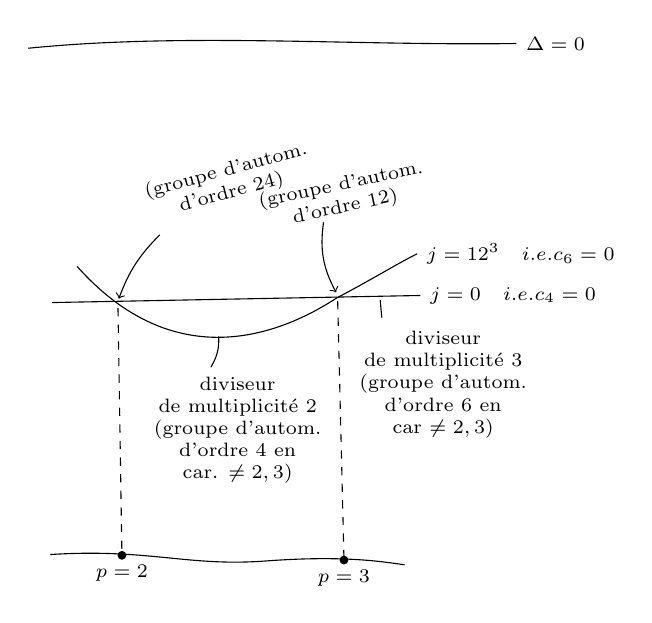
\begin{tikzpicture}[x=1cm,y=1cm,font=\scriptsize]
\draw (0,6.9) .. controls (2,7.1) and (4.1,6.93) .. (6.2,6.96) node[right] {$\Delta=0$};
\draw (0.3,3.67) -- (4.98,3.76) node[right] {$j=0\quad\text{i.e. }c_4=0$};
\draw (0.62,4.13) .. controls (1.83,2.77) and (3.14,3.22) .. (3.92,3.73)
 .. controls (4.34,3.95) and (4.68,4.16) .. (4.94,4.29)
 node[right] {$j=12^3\quad\text{i.e. }c_6=0$};
\draw[->] (1.67,4.53) to[bend right=12] (1.15,3.72);
\node[rotate=15,align=center,anchor=south west] at (1.50,4.52)
 {(groupe d'autom.\\d'ordre 24)};
\draw[->] (3.75,4.69) to[bend right=18] (3.91,3.80);
\node[rotate=12,align=center,anchor=south] at (4.08,4.64)
 {(groupe d'autom.\\d'ordre 12)};
\draw (2.42,3.24) to[bend left=16] (2.32,2.85);
\node[align=center,anchor=north] at (2.66,2.85)
 {diviseur\\de multiplicité 2\\(groupe d'autom.\\d'ordre 4 en\\car. $\ne2,3$)};
\draw (4.47,3.70) -- (4.49,3.48);
\node[align=center,anchor=north] at (5.27,3.43)
 {diviseur\\de multiplicité 3\\(groupe d'autom.\\d'ordre 6 en\\car $\ne2,3$)};
\draw[dashed] (1.14,3.60) -- (1.19,.46);
\draw[dashed] (3.93,3.69) -- (4.01,.40);
\draw (.28,.47) .. controls (1.55,.55) and (2.03,.31) .. (3.04,.39) .. controls (4.02,.46) and (4.49,.38) .. (4.78,.34);
\fill (1.19,.46) circle (1.6pt) node[below] {$p=2$};
\fill (4.01,.40) circle (1.6pt) node[below] {$p=3$};
\end{tikzpicture}}

\[
\deleted{\unsure{j}}\quad
\left\{\begin{aligned}
 \operatorname{div}(j)^+&=3\operatorname{div}(c_4)&\tfrac13\operatorname{div}(j)^+&=\operatorname{div}c_4\\
 \operatorname{div}(j)^-&=M^{(\infty)}\\
 \operatorname{div}(j-12^3)^+&=2\operatorname{div}(c_6)&\tfrac12\operatorname{div}(j-12^3)^+&=\inserted{\operatorname{div}c_6}\\
 \operatorname{div}(j-12^3)^-&=M^{(\infty)}\\
 M^{(\infty)}&=\operatorname{div}\Delta
\end{aligned}\right.
\]
\[
\left\{\begin{aligned}
 \operatorname{cl}\deleted{\unsure{\operatorname{div}}}\bigl(\tfrac13\operatorname{div}(j)^+\bigr)&=\omega^4\\
 \operatorname{cl}\bigl(\tfrac12\operatorname{div}(j-12^3)^+\bigr)&=\omega^6\\
 \operatorname{cl}(M^\infty)&=\omega^{12}
\end{aligned}\right.
\]
\hrule

Sous-site étale \inserted{$\deleted{\unsure{M}}V(c_4)=M'$} du site modulaire $\deleted{\unsure{\mathcal M}}M$ défini par l'équation $c_4=0$

a) Dans le \deleted{complémentaire} ouvert $(M'_{/6}=M'\,|\,\underbrace{(\operatorname{Spec}\mathbb Z-\{2\}-\{3\}}_{\operatorname{Spec}\mathbb Z[\frac16]})$, c'est isomorphe à $\deleted{\unsure{\operatorname{Spec}\mathbb Z[\tfrac16]}}\ B_{\mu_6}\,|\,\operatorname{Spec}\mathbb Z[\tfrac16]$ ; on peut \deleted{\unsure{se|le}} décrire \deleted{\unsure{canoniquement|comme isom.}} ces courbes \deleted{\unsure{de genre 1}}\inserted{elliptiques} sur $S$, avec $c_4=0$ (\unsure{où|si} $6$ inv. sur $S$) comme les torseurs sous $\mu_6$ ; à $E$ correspond le torseur de ses isom. avec la courbe d'équation \unsure{non} homogène $y^2=x^3+1$. [ NB. Il y a en tout $72$ courbes elliptiques sur $\mathbb Z[\frac16]$ avec $c_4=0$, car
\[
 H^1(\operatorname{Spec}\mathbb Z[\tfrac16],\mu_6)\simeq
 \deleted{\unsure{\mathbb Z_{/6\mathbb Z}\times\mathbb Z_{/6}\ \operatorname{Spec}}}
 \bigl(\mathbb Z[\tfrac16]\bigr)^*_{6}\simeq
 \mathbb Z_{/6\mathbb Z}\times\mathbb Z_{/6\mathbb Z}\times\mathbb Z_{/2\mathbb Z}
\]

b) La fibre de $M'$ en $p=2$ est de \deleted{\unsure{ordre 4}} multiplicité 4 en chaque point, en $p=3$ est de multiplicité 2. Donc $M'$ est ramifié sur $\mathbb Z$ \inserted{exactemt} en l'unique point au dessus de $p=2$ et l'unique point au dessus de $p=3$.

$M'$ est-il \uline{régulier} ?? \uuline{Non}, pas en $p=2$ \deleted{\unsure{et}}, mais régulier en $p=3$.

\smallskip\noindent\rule{.30\linewidth}{.3pt}

Sous-site étale $V(c_6)=M''$ du site modulaire.

a) Dans l'ouvert $(M''_{/6}=M''\,|\,\operatorname{Spec}\mathbb Z[\tfrac16],=M''-M''_{(2)}-M''_{(3)}$, c'est $\simeq B_{\mu_4}\,|\,\operatorname{Spec}\mathbb Z[\tfrac16]$.

(il y a $\unsure{-|=}$32 \unsure{courbe|courbes} elliptiques avec $c_6=0$ sur $\mathbb Z[\frac16]$, qu'on peut choisir comme origine \ldots)

b) $M''_{(2)}$ est de multiplicité 6, $M''_{(3)}$ est de multiplicité 3, Donc $M''$ est ramifié sur $\mathbb Z$ \unsure{exactemt} en l'unique pt sur $p=2$ et l'unique point sur $p=3$.

$M''$ est-il régulier ?? \uuline{Non}, pas en $p=2,3$ !
% archive sheet number: 95
\scanpage{97}
% The letter is inverted relative to the scan. Three long strokes cancel the sheet.
\deleted{Wattignies $9/\overline{\underline{\mathrm{III}}}/68$.}\\

\deleted{Cher Monsieur Grothendieck.}\\

\deleted{Je vous suis trés reconnaissant des démarches \unsure{au près|auprès} de M\textsuperscript{r}. Verdier et M\textsuperscript{r} Deligne. Je parlerai avec Monsieur Deligne d\unsure{ès|és} que j'aurais fini la lecture du séminaire Hartshorne comme vous me le conseillez.}

\deleted{Merci bien enfin pour votre lettre, de même que les papiers du Seminaire. Le problème de définir les \unsure{operations|opérations} $\unsure{\wedge^{i}|\Lambda^{i}}$ m'a interessé. J'en parlerais à Monsieur Deligne.}

\deleted{Je vous envoie, Monsieur Grothendieck, mes}\\
\deleted{meilleures salutations.}\\

\deleted{Carlos \unsure{Ruir|Ruiz} S.}\\
% archive sheet number: 96
\scanpage{98}
Donc il s'ensuit que $M_3\deleted{\unsure{[1/3]}}\cap V(c_4)$ a exactement 4 composantes irréductibles, \deleted{\unsure{elles}} qui ne peuvent se rencontrer qu'au dessus du point $p=2$. Il y a \unsure{évidemt} 1 composantes connexes, car la fibre de $M_3[1/3]$ au dessus de l'unique point de $\mu_3^*$ sur $p=2$ [qui correspond au \deleted{\unsure{$\mathbb F$}} corps résiduel $\mathbb F_4=\mathbb F_2(\sqrt[3]{1})$] est de \deleted{degré} rang géom. 1. Cela provient du fait que le \unsure{gpe} des \unsure{autom.} d'une \unsure{c.} $E$ en car. 2 \inserted{(sur corps alg clos)} avec $c_4=0$, est $\mathrm{Sl}(2,\mathbb Z/3\mathbb Z)$, \deleted{qui agit \unsure{transitivement} sur l'ens des \unsure{toutes} les bases}\inserted{et l'\unsure{ens|aire|une} des orbites sous ce groupe de l'ens des \deleted{toutes} les} bases de $\mathord{}_3E$ est deux.

\figure{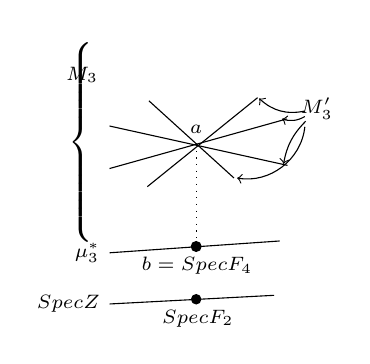
\begin{tikzpicture}[x=1cm,y=1cm,font=\scriptsize]
\node at (-.35,3.15) {$M_3$}; \node at (-.35,2.33) {\(\left\{\rule{0pt}{1.4cm}\right.\)};
\draw (0,1.96)--(2.25,2.59); \draw (0,2.50)--(2.26,2.00);
\draw (.48,1.73)--(1.88,2.86); \draw (.50,2.82)--(1.58,1.84);
\node[above] at (1.1,2.28) {$a$};
\node at (2.63,2.72) {$M'_3$};
\draw[->] (2.48,2.69) to[bend left=27] (1.90,2.85);
\draw[->] (2.48,2.62) to[bend left=23] (2.19,2.59);
\draw[->] (2.49,2.56) to[bend right=17] (2.21,2.02);
\draw[->] (2.48,2.49) to[bend left=47] (1.62,1.84);
\draw[dotted] (1.10,2.27)--(1.10,.93);
\draw (0,.89)--(2.16,1.04); \fill (1.10,.97) circle (2pt);
\node[left] at (0,.89) {$\mu_3^*$}; \node[below] at (1.11,.96) {$b=\operatorname{Spec}\mathbb F_4$};
\draw (0,.24)--(2.09,.35); \fill (1.10,.30) circle (1.9pt);
\node[left] at (0,.24) {$\operatorname{Spec}\mathbb Z$}; \node[below] at (1.12,.29) {$\operatorname{Spec}\mathbb F_2$};
\end{tikzpicture}}

\deleted{\unsure{qui sont}} La courbe $\unsure{\mathbb E|E|\overline E}$ \deleted{\unsure{se descend évidemment}}\inserted{a bonne réduction} sur \inserted{tout} l'anneau des entiers \deleted{\unsure{des}} corps de $\mu_3^*$, \unsure{ou|sur} $\mathbb Q(\sqrt[3]{1})$, \deleted{Il y a} sans exclure 2 (ni 3 ?). Comme $\deleted{\unsure{V'}}M_3^{\unsure{*|2}}\deleted{\unsure{[1/3]}}$ et à fortiori $M_3\cap V(c_4)$ est au dessus de $\mu_3^*[\frac13]$, il s'ensuit que les composantes irréductibles (qui sont entières sur $\mu_3^*[\frac13]$ et \unsure{birationelles|birationnelles} sur lui) sont \uline{identiques} à $\mu_3^*[\frac13]$. Donc chacune des \unsure{restrictions} de la courbe \inserted{elliptique} universelle sur $M_3$ aux composantes irréductibles de $\mu_3^*[\frac13]$ sont isomorphes à $\mathbb E$ envisagé plus haut (ou plutôt, son extension canonique à $\mu_3^*[\frac13]$ -- on voit qu'elles se réduisent bien aussi au point $p=2$), mais avec des 3-rigidifications différentes. Le raccord des quatre composantes se fait d'abord \unsure{$\circ$}
% slanted
\margin{\unsure{$\circ$} grâce au fait que les fibres de \unsure{ces} $E^{(i)}$ en $a$ \unsure{s.t|st|et à} (de façon unique) isomorphes comme courbes elliptiques \uline{rig.} d'échelon 3 ; mais le \unsure{raccordement|raisonnement|raccord|second énoncé} est encore trop lâche \ldots\ldots}

A examiner si les \deleted{tangentes} 4 composantes de $M'_3$ en le point $a$ de $(M'_3)_2$ \deleted{sont} ``à tangentes distinctes'' ; comme le corps résiduel est $\mathbb F_4$, et que $\operatorname{card}\mathbb P^1_{\mathbb F_4}=5$, dont il faut enlever la verticale, cela \uline{signifierait} que les tangentes épuisent toutes les classes non verticales de l'espace tangent de Zariski en $a$. Or ces tangentes sont transformées \inserted{l'une de l'autre} par \unsure{l'opérations|les opérations} de $G'=\mathrm{Sl}(2,\mathbb Z_{/3\mathbb Z})$. [qui est le \unsure{un} groupe d'inertie \unsure{du|en} $a$, est un groupe de \deleted{\unsure{$\mathbb F$ ou}} \unsure{$\mu_3^*\!{}_{T_a}$-autom|$\mu'_3$-autom} de] \deleted{le groupe qui laisse} Comment opère-t-il sur l'espace tangent de Zariski \inserted{de} en $a$ ? \deleted{qui} Il doit laisser invariant l'application $T_a\to T_b$, \deleted{donc le} (car op. trivialemt sur $T_b$) donc opère via $\mathbb F_4^*\cdot\mathbb F_4$.
\margin{sur $\unsure{\mathbb F_3|\mathbb F_4}$ \quad $\begin{pmatrix}*&*\\0&1\end{pmatrix}$}
Notons que $B'$ \deleted{\unsure{opè}} laisse chaque composante irréductible invariante, donc \deleted{laisse invariante leurs \unsure{espaces}}\inserted{opère trivialemt, donc opère} \deleted{\unsure{sur}} \inserted{trivialt sur l'espace} \deleted{tangent} de Zariski ; \deleted{donc $B'$ opère} s'il y en avait deux distinctes, il opérerait aussi trivialement sur l'espace tangent de Zariski de $M_3$ en $a$, mais alors (comme le ss. gpe inv. de $G'$ engendré par $B'$ est $G'$) \deleted{$G'$ \unsure{est}} \deleted{il \unsure{engendrerait}} opérant trivialement, et comme il est transitif] sur l'ens des tangentes des composantes de $M'_3$ en $a$, on aurait contradiction. \uline{Donc les quatre}
% archive sheet number: 97
\scanpage{99}
% archive sheet number: 98

\uline{Paramètres locaux} \uline{du site modulaire} :

a$'$) Dans le complémentaire de $M'\cup M''\cup M^\infty$ $\left(\underset{\substack{|\\c_4=0}}{j=0},\,\underset{\substack{|\\c_6=0}}{j=12^3},\,\underset{\substack{|\\\Delta=0}}{j=\infty}\right)$ \deleted{est} \deleted{\unsure{on|la}} on peut prendre la fonction $j$

\deleted{\unsure{a)|b)}} Dans le complémentaire de $M'\cup M''$, on peut prendre $1/j$ ou $\dfrac{1}{j-12^3}$.

\deleted{b) Dans le complémentaire de}

b) Au voisinage de $(M')_6$, on peut prendre $c_4$.

c) \rule{4em}{.3pt} $(M'')_6$, \rule{4em}{.3pt} $c_6$.

d) Au voisinage du point $p=2$, $c_4=0$, $c_6=0$ on peut prendre $a_1$

e) Au voisinage du point $p=3$, $c_4=0$, $c_6=0$ \rule{4em}{.3pt} $b_2$

\uline{Question} Donner la structure de l'anneau local complété de $M$ en un point géom. où $c_4=0$, $c_6=0$ [il y en a \deleted{\unsure{essentiellement}]}\ deux : \unsure{Bien|Bon} \unsure{sûr|pris}, l'un en car. $2$, l'autre en car. $3$]
\[
\deleted{\unsure{A=|R=}}\,\underset{\substack{|\\\text{corps résiduel}\\\text{clôture algébrique}\\\text{de }\mathbb F_2\ \text{resp. }\mathbb F_3}}{W}[[t]]
\qquad (t=a_1\ \text{en car. }2,\quad t=b_2\ \text{en car. }3)
\]
et les équations des diviseurs $c_4=0$, $c_6=0$ \ldots..

\noindent\rule{\linewidth}{.3pt}

\margin{$\left.\begin{gathered}
G\ \text{d'ordre }48\\
B\ \text{d'ordre }12\\
G/B\ \text{d'ordre }4\\
B/\mu_6\ \text{d'ordre }2\simeq\mu_2\\
\mu_6=\underbrace{\mu_2}_{\substack{\Vert\\\text{centre}\\ Z}}\times\underbrace{\mu_3}_{\substack{\Vert\\\unsure{B_u|Bu}}},\\
G'=\mathrm{Sl}(2,\mathbb Z/3\mathbb Z),\ B'=G'\cap B\\
G'/B'\ \text{d'ordre }4\ldots\\
G'\ \text{d'ordre }24\\
B'\ \text{d'ordre }6
\end{gathered}\right\}$}
% slanted

Étudions la structure de $V(c_4)$ dans $(M_3)$. On trouve que si $E$ est une courbe elliptique sur $S$, avec $6$ inv. sur $S$ et $c_4(E)=0$, alors ds $\mathord{}_3E$ il y a un unique drapeau invariant par $\underline{\mathrm{Aut}}_S(E)\simeq\mu_6$. Ceci permet de ``réduire le groupe structural'' $G=\mathrm{Gl}(2,\mathbb Z/3\mathbb Z)$ de $(M_3)[1/6]$ de $G$ à $B$ (le Borel). On trouve que sur $\underline S=\mu_3^*[\frac16]$ (schéma des racines primitives 3ièmes de $1$), \deleted{\unsure{qui comprend|qui}} il y a une courbe elliptique $\mathbb E$ avec $c_4(E)=0$, et une base $e_1^0,e_2^0$ adaptée au drapeau précédent, $\langle e_1^0,e_2^0\rangle=\zeta^0$ (où $\zeta^0$ est la racine 3ième de l'unité canonique) ; cette $\overline E$ est définie à isom. unique près. Toute courbe elliptique \inserted{$E$} sur $S$, avec rigidification \inserted{$e_1,e_2$} d'échelon 3, définit un $S\longrightarrow\underline S$ (\unsure{après|grâce à} : $\zeta=\langle e_1,e_2\rangle$), \deleted{et} $E$ est isomorphe à $\overline E\times_{\underline S} S$, avec \inserted{(loc.)} soit la rigidification \unsure{image inverse}, soit \deleted{la rigidification}\inserted{une des trois autres} qui s'en déduisent par translation par élmt de $G$ \unsure{mod.|m. de|mod} $B$. Donc $M_3[1/6]\cap V(c_4)$ est isomorphe à la somme de $4$ copies de $\mu_3^*[\frac16]$, et est can. isom. à $\mu_3^*(1/6)\deleted{\unsure{\times}} \mathbin{\overset B\times}G$, comme espace où $G$ opère ($B$ opère sur $\mu_3^*$ via déterminant). T.S.V.P.
\scanpage{100}

Tangentes \inserted{aux composantes irréductibles} de $M'_3$ \uline{en $a$} sont \deleted{\unsure{distinctes}} égales. \deleted{$G'$ \unsure{opère sur}} \inserted{L'espace} tangent à $M_3$ en $a$ splitte canoniquement en $V_1\times V_2$, avec $V_1$ vertical (espace tangent à $(M_3)_b$) et $V_2$ horizontal, et $G'$ opère \unsure{trivialemt|trivialem} sur $V_2$, et laisse $V_1$ stable. donc $G'$ opère via $\mathbb F_4^*\inserted{\simeq\mathbb Z/3\mathbb Z}$ sur $V_1$. Or, \deleted{\unsure{la|les}} théorie de la ramification en car. 2 nous dit précisément [l'action de $G'$ sur $(M_3)_2$ étant \deleted{\unsure{fidèle, que}}\inserted{fidèle}) que le noyau de \deleted{la partie stable de} \unsure{ordres|est très} vraisemblablement précisément le 2-sous-groupe invariant \inserted{$P'$} de $G'$, qui est d'ordre 8, \deleted{\unsure{et dès}} que l'image \deleted{\unsure{étant}} \unsure{être|est} d'ordre \deleted{\unsure{card}} $[G':P']=3=\operatorname{card}\mathbb F_4^*\simeq\mathbb Z/3\mathbb Z$. Par suite, on trouve que $G'\to\mathbb F_4^*$ est surjectif, et déterminé à priori ``au signe près'' [i.e via autom. du \inserted{groupe} $\mathbb Z/3\mathbb Z$] Il faudrait encore déterminer lequel\deleted{\unsure{lement|que}} c'est.

\margin{\figure{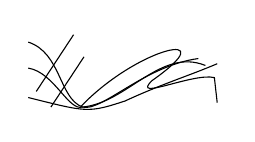
\begin{tikzpicture}[x=.6cm,y=.55cm]
\draw (0,1.5) .. controls (.7,1.25) and (.65,.2) .. (1.15,0) .. controls (1.55,-.12) and (2.45,.95) .. (3.6,1.12);
\draw (0,.9) .. controls (.55,.8) and (.85,-.1) .. (1.15,0) .. controls (2.1,.1) and (2.8,1.38) .. (3.75,.96);
\draw (0,.22) .. controls (1.25,-.12) and (1.26,-.14) .. (2.05,.14) .. controls (2.82,.53) and (3.42,.73) .. (4,1);
\draw (.17,.36)--(.96,1.67) (.48,0)--(1.18,1.16) (1.12,.02).. controls (2.36,1.42) and (4.2,1.82)..(2.62,.61).. controls (2.16,.12) and (3.5,.8)..(3.94,.68)--(4,.1);
\end{tikzpicture}}}

\uline{Attention}, $\mu_3$ \uuline{n'opère pas} sur la courbe modulaire $\mathbb E$ sur $M'_3$, \deleted{en s'y \unsure{opérant}} \inserted{en prolongeant son} action au dessus de $M'_3[\frac13]$. Car \deleted{\unsure{alors on}} son \deleted{\unsure{en remarquant que son action sur}} action commuterait à celle de $G$, \deleted{\unsure{donc} qui \unsure{serait} l'action résiduelle par $\mu_6$ \unsure{serait}, donc fidèle en tt point, \unsure{on en sait que|ce fait sait que} le gpe des autom. \deleted{\unsure{est}} à fibres étales, donc sa fibre chez le point 2 un point \unsure{contient} $\mu_6=\underset{\text{radical}}{\mu_2}\times\mu_3$. Par contre, \inserted{$=\mu_6$} $\mu_3$ opère sur la $\mathbb Z/6\mathbb Z=B$ opère sur \unsure{$E$} tte \unsure{courbe} elliptique en opérant sur \unsure{$E$} \unsure{au de façon} canoniquement pour la \unsure{raison}, $E$ sur une base de car. résiduelle $\ne3$,} donc on a on aurait action de $\mu_3$ et $G'$ sur $E_a$, et comme $G'=\mathrm{Aut}(E_a)$, il s'ensuivrait que $\mu_3\subset G'$ est $\mu_3$ dans le centre de $G'$. Or le 3-sous-groupe de Sylow \deleted{\unsure{du}} de $G'$ \uline{n'est pas central} ! // Ceci impose des restrictions \deleted{\unsure{sur les}}\inserted{aux} raccords des composantes de $M'_3$. \deleted{\unsure{La seule}} \inserted{groupe des} autom. \unsure{automorphismes} de $E$ sur $M'_3$ est donc $\mathbb Z/2\mathbb Z$, \unsure{par} \deleted{$\mathrm{Sl}(2,\unsure{\mathbb Z/3\mathbb Z})/\unsure{\mu_2|\mu_3}$ \unsure{opère fidèlement sur} $M'_3$} qui est aussi le grpe noyau de \deleted{\unsure{sur}} l'opération de $\mathrm{Sl}(2,\mathbb Z/3\mathbb Z)=G'$, sur $M'_3$.

\margin{\figure{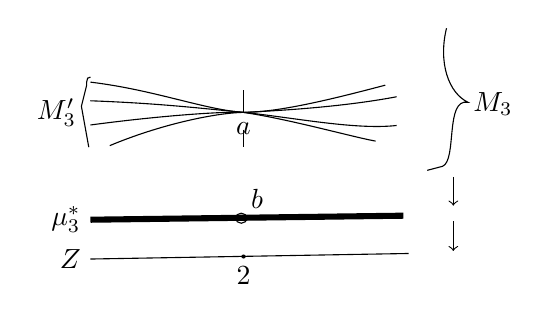
\begin{tikzpicture}[x=.72cm,y=.64cm]
\draw (0,2.82).. controls (1.12,2.67) and (2.02,2.27)..(2.7,2.22).. controls (3.36,2.22) and (4.42,2.53)..(5.2,2.76);
\draw (0,2.45).. controls (1.22,2.40) and (1.95,2.3)..(2.7,2.22).. controls (3.65,2.27) and (4.6,2.36)..(5.4,2.53);
\draw (0,1.97).. controls (1.2,2.15) and (2.3,2.24)..(2.7,2.22).. controls (3.62,2.11) and (4.68,1.87)..(5.4,1.96);
\draw (.34,1.56).. controls (1.23,1.98) and (2.2,2.21)..(2.7,2.22).. controls (3.53,2.08) and (4.63,1.73)..(5.03,1.65);
\draw (2.7,2.66)--(2.7,2.23) (2.7,1.88)--(2.7,1.54);
\node[below] at (2.7,2.22){$a$};
\draw (0,2.92).. controls (-.1,2.94) and (-.05,2.73)..(-.08,2.7)--(-.16,2.34)--(-.03,1.53);
\node[left] at (-.08,2.22){$M'_3$};
\draw (6.28,3.89).. controls (6.13,3.2) and (6.32,2.6)..(6.66,2.42).. controls (6.25,2.51) and (6.47,1.27)..(6.21,1.15)--(5.94,1.07);
\node[right] at (6.58,2.38){$M_3$};
\draw[line width=2.2pt] (0,.09)--(5.52,.17);
\draw (2.66,.12) circle (.1);
\node[above right] at (2.66,.12){$b$};
\node[left] at (0,.09){$\mu_3^*$};
\draw (0,-.69)--(5.61,-.58);
\fill (2.70,-.64) circle (.04);
\node[below] at (2.70,-.64){$2$};
\node[left] at (0,-.69){$\mathbb Z$};
\draw[->] (6.4,.94)--(6.4,.37);
\draw[->] (6.4,.06)--(6.4,-.53);
\end{tikzpicture}}}
% archive sheet number: 99
\scanpage{101}
% Two long oblique strokes run down across the typescript; the first begins at « pour ».
\deleted{pour lesquels l'expression $(*)$ est définie.}

\deleted{fermé $Z_s$ de $X_s$, où $Z$ est le sous-schéma fermé de $X$ adhérence \deleted{\unsure{de}}schématique de $Z_t$ (de sorte que $Z$ est le sous-schéma fermé intègre de $X$ défini par l'adhérence topologique de $Z_t$). \deleted{Je dis} \inserted{Il faudrait montrer} que cet homomorphisme passe au quotient pour définir un homomorphisme d'anneaux gradués}
\[
\deleted{\mathord{:}\ A^{\bullet}(X_t)\qquad A^{\bullet}(X_s)\quad .}\tag*{(7.11.2)}
\]

\deleted{Pour montrer que (7.10.1) transforme cycles linéairement équivalents à zéro en cycles linéairement équivalents à zéro, on introduit le schéma $C=P^1_S$, les deux sections $x_{\unsure{o|0}}$ et $x_1$ de $C$ sur $S$ définies par $0$ et $1$, et on se rappelle que le groupe des cycles \unsure{linéairement|linéairment} équivalents à zéro sur $X_t$ est engendré par les cycles}
\[
\deleted{Z_t(x_{1t})\ \deleted{\unsure{=|\times}}\unsure{-|=}\ Z_t(x_{ot})\ ,}\tag*{$(*)$}
\]
\deleted{où $Z_t$ parcourt le\deleted{s cycles} groupe des cycles sur $X_t\mathbin{\mathrm{x}}_{k(t)}C_t$\handwritten{\unsure{!}}. Or un calcul d'intersections facile (\hspace{3em}) montre que l'image par (7.11.1) du cycle $(*)$ n'est autre que}
\[
\deleted{Z_s(x_{1s})-Z_s(x_{os})\quad ,}\tag*{$(*\ *)$}
\]
\deleted{où $Z$ désigne encore l'adhérence schématique de $Z_t$ dans $X$, \uline{pourvu que l'expression} $(*\ *)$ \uline{soit définie}.}
% archive sheet number: 100
